%
% umkehrformel.tex
%
% (c) 2019 Prof Dr Andreas Müller, Hochschule Rapperswil
%
\begin{frame}
\frametitle{Umkehrformel für $\mathbb R^n$}
Gegeben: $\mathcal{B}=\{\vec{b}_1,\dots,\vec{b}_n\}\subset\mathbb R^n$
orthonormierte Basis, d.~h.
\[
\langle \vec{b}_j,\vec{b}_i\rangle = \delta_{ji}
\]
\uncover<2->{%
Koordinaten eines Vektors $\vec{v}$ in der Basis
\[
	v_i = \langle \vec{v},\vec{b}_i\rangle
\]
}
\uncover<3->{%
Rekonstruktion:
\[
\vec{w}
=
\sum_{j=1}^{n} v_j\vec{b}_j
\uncover<4->{%
=
\sum_{j=1}^n \langle \vec{v},\vec{b}_j\rangle \vec{b}_j}
\]
}
\uncover<5->{%
Verifikation: $\vec{w}$ hat die gleichen Koordinaten wie $\vec{v}$
\begin{align*}
\uncover<6->{\langle \vec{w},\vec{b}_i\rangle}
&\uncover<7->{=\biggl\langle
\sum_{j=1}^n \langle \vec{v},\vec{b}_j\rangle\vec{b}_j, \vec{b}_i
\biggr\rangle}
\uncover<8->{=
\sum_{j=1}^n \langle \vec{v},\vec{b}_j\rangle \langle \vec{b}_j,\vec{b}_i\rangle}
\uncover<9->{=
\sum_{j=1}^n \langle \vec{v},\vec{b}_j\rangle \delta_{ji}}
\uncover<10->{=
\langle \vec{v},\vec{b}_i\rangle}
\uncover<11->{\quad{\color{red}\checkmark}}
\end{align*}
}

\end{frame}

%
% Vermutung für Umkehrformel für CWT
%
\begin{frame}
\frametitle{Umkehrformel für CWT}
\begin{cwt}
Wavelet-Transformierte von $f\in L^2(\mathbb R)$:
\[
\mathcal{W}f(a,b)
=
\frac{1}{\sqrt{|a|}}
\int_{-\infty}^\infty f(t) \overline{\psi\biggl(\frac{t-b}{a}\biggr)} \,dt
\uncover<2->{=
\langle f,\psi_{a,b}\rangle}
\]
\end{cwt}
\uncover<3->{%
Analyse mit
\begin{itemize}
\item<4->
$L^2$-Skalarprodukt
\item<5->
``Basis'': $T_bD_a \psi = \psi_{a,b}$
\end{itemize}
}
\uncover<6->{%
\begin{umkehrformel}
\ifthenelse{\boolean{presentation}}{
\only<6>{%
Für $\vec{v}\in \mathbb R^n$ mit Basis
$\mathcal{B}=\{\vec{b}_1,\dots,\vec{b}_n\}$
}
\only<7>{%
Für $f\in L^2$ mit Basis
$\mathcal{B}=\{\vec{b}_1,\dots,\vec{b}_n\}$
}
\only<8-13>{%
Für $f\in L^2$ mit ``Basis''
$\psi_{a,b}$:
}
\only<14->{für $\mathcal{W}f(a,b)$:\phantom{$L^2$ mit ``Basis''}}
\[
\only<6>{
\vec{v}=\sum_{j=1}^\infty \langle \vec{v},\vec{b}_j\rangle\,\vec{b}_j
}
\only<7>{
f=\sum_{j=1}^\infty \langle f,\vec{b}_j\rangle\, \vec{b}_j
}
\only<8>{
f=\sum_{a,b}^{\phantom{\infty}} \langle f,\psi_{a,b}\rangle\, \psi_{a,b}
}
\only<9>{
f=\sum_{a,b}^{\phantom{\infty}} \mathcal{W}f(a,b)\,\psi_{a,b}
}
\only<10>{
f(t)=\sum_{a,b}^{\phantom{\infty}} \mathcal{W}f(a,b)\,\psi_{a,b}(t)
}
\only<11>{
f(t)=\sum_{a}^{\phantom{\infty}} \int_{-\infty}^\infty \mathcal{W}f(a,b)\,\psi_{a,b}(t)\, db
}
\only<12>{
f(t)=\int_{\mathbb R^+} \int_{-\infty}^\infty \mathcal{W}f(a,b)\psi_{a,b}(t)\, db \,da
}
\only<13>{
f(t)=\int_{\mathbb R^+} \int_{-\infty}^\infty \mathcal{W}f(a,b)\psi_{a,b}(t)\, db \,\frac{da}{|a|^2}
}
\only<14>{
f(t)
\stackrel{{\color{red}?}}{=}
\int_{\mathbb R^+} \int_{-\infty}^\infty \mathcal{W}f(a,b)\psi_{a,b}(t)\, db \,\frac{da}{|a|^2}
}
\]}{
\[
f(t)
\stackrel{{\color{red}?}}{=}
\int_{\mathbb R^+} \int_{-\infty}^\infty \mathcal{W}f(a,b)\psi_{a,b}(t)\, db \,\frac{da}{|a|^2}
\]
}
\end{umkehrformel}
}
\end{frame}

%
% Verifikation der Umkehrformel
%
\begin{frame}
\frametitle{Vergleichsprinzip}

\begin{vergleich}
Für zwei Funktionen $f_1$ und $f_2$ in $L^2(\mathbb R)$ gilt
\[
\left.
\begin{aligned}
f_1&=f_2
&&\Leftrightarrow&
\langle f_1,g\rangle &= \langle f_2,g\rangle
\\
f_1-f_2&=0
&&\Leftrightarrow&
\langle f_1-f_2,g\rangle &= 0
\end{aligned}
\quad\right\}
\quad
\text{für alle $g\in L^2(\mathbb R)$}
\]
\end{vergleich}
\vspace*{-10pt}

\begin{proof}[Beweis]
Richtung $\boxed{\Rightarrow}$\;: Verwende Cauchy-Schwarz-Ungleichung
\begin{align*}
f_1&=f_2
&&\Rightarrow&
f_1-f_2&=0
&&\Rightarrow&
|\langle f_1-f_2,g\rangle|
&\le
\underbrace{\|f_1-f_2\|}_{\displaystyle=0}\cdot \|g\|
\end{align*}
\vspace{-20pt}

Richtung $\boxed{\Leftarrow}$\;: Verwende $g=f_1-f_2$
\begin{align*}
\langle f_1-f_2,g\rangle&=0
&&\Rightarrow&
\|f_1-f_2\|
&=
\langle f_1-f_2,f_1-f_2\rangle
=
0
&&\Rightarrow&
f_1-f_2&=0
\end{align*}
\end{proof}

\end{frame}

%
% Verifikation der Umkehrformel
%
\begin{frame}
\frametitle{Verifikation der Umkehrformel $\mathbb R^n$}
Umkehrformel muss gleiche Skalarprodukte mit $\vec{w}$ haben wie $\vec{v}$:
\[
\langle \vec{v},\vec{w}\rangle
\stackrel{?}{=}
\langle \text{Umkehrformel für $\vec{v}$},\vec{w}\rangle
\qquad\text{für alle $\vec{w}\in\mathbb R^n$}
\]
\uncover<2->{
Nachrechnen
\begin{align*}
&\hbox to8cm{\hfill}\\[-20pt]
\langle\vec{v},\vec{w}\rangle
&\stackrel{?}{=}
\ifthenelse{\boolean{presentation}}{
\only<3>{
\biggl\langle
\sum_{j=1}^n \langle \vec{v},\vec{b}_j\rangle\,\vec{b}_j,\vec{w}
\biggr\rangle
}
\only<4>{
\sum_{j=1}^n \langle \vec{v},\vec{b}_j\rangle\,\langle\vec{b}_j,\vec{w}\rangle
}
\only<5>{
\sum_{j=1}^n \langle \vec{v},\vec{b}_j\rangle\,
\overline{\langle\vec{w},\vec{b}_j\rangle}
}
\only<6->{
\sum_{j=1}^n v_j\bar{w}_j
}
\only<7->{
\qquad\text{Parseval-/Plancherel-Formel}
}}{
\sum_{j=1}^n v_j\bar{w}_j
\qquad\text{Parseval-/Plancherel-Formel}
}
\end{align*}
\uncover<8->{%
\begin{parseval}
$f,g$ $2\pi$-periodische Formeln mit Fourierkoeffizienten 
$a_k^f,a_k^g$ und $b_k^f,b_k^g$, dann gilt
\vspace{-10pt}

\[
\langle f,g\rangle
=
\frac12
a_0^f \overline{a_0^g}
+
\sum_{k=1}^\infty
(
a_k^f \overline{a_k^g}
+
b_k^f \overline{b_k^g}
)
\]
\end{parseval}}
}
\vspace*{-10pt}
\uncover<9->{%
\begin{plancherel}
Für $f,g\in L^2(\mathbb R)$ gilt
\[
\langle f, g\rangle
=
\langle \mathcal{F}f,\mathcal{F}g\rangle
=
\langle \hat{f},\hat{g}\rangle
\]
\end{plancherel}}

\end{frame}

%
% Verifikation der Umkehrformel
%
\begin{frame}
\frametitle{Verifikation der Umkehrformel $\mathcal{W}f$}

Umkehrformel muss gleiche Skalarprodukte mit $g$ haben wie $f$:
\[
\langle f,g\rangle
\stackrel{?}{=}
\langle \text{Umkehrformel für $f$},g\rangle
\qquad\text{für alle $g\in L^2$}
\]
\uncover<2->{
Nachrechnen
\begin{align*}
&\hbox to8cm{\hfill}\\[-20pt]
\langle f, g\rangle
&
\stackrel{?}{=}
\ifthenelse{\boolean{presentation}}{
\only<3>{
\biggl\langle
\int_{\mathbb R^+}\int_{-\infty}^\infty
\mathcal{W}f(a,b)\,\psi_{a,b}
\, db\,\frac{da}{|a|^2},
g
\biggr\rangle}
\only<4>{
\int_{-\infty}^\infty
\int_{\mathbb R^+}\int_{-\infty}^\infty
\mathcal{W}f(a,b)\,\psi_{a,b}(t)
\, db\,\frac{da}{|a|^2}
\,
\overline{g(t)}
\,dt
}
\only<5>{
\int_{\mathbb R^+}\int_{-\infty}^\infty
\mathcal{W}f(a,b)
\int_{-\infty}^\infty
\psi_{a,b}(t)
\,
\overline{g(t)}
\,dt
\, db\,\frac{da}{|a|^2}
}
\only<6>{
\int_{\mathbb R^+}\int_{-\infty}^\infty
\mathcal{W}f(a,b)
\langle
\psi_{a,b},
g
\rangle
\, db\,\frac{da}{|a|^2}
}
\only<7>{
\int_{\mathbb R^+}\int_{-\infty}^\infty
\mathcal{W}f(a,b)
\overline{
\langle
g,
\psi_{a,b}
\rangle}
\, db\,\frac{da}{|a|^2}
}
\only<8-10>{
\int_{\mathbb R^+}\int_{-\infty}^\infty
\mathcal{W}f(a,b)
\overline{\mathcal{W}g(a,b)}
\, db\,\frac{da}{|a|^2}}
\only<11->{
\langle 
\mathcal{W}f(a,b),
\mathcal{W}g(a,b)
\rangle_H}
\only<12->{\qquad\text{Plancherel-Formel}}}{
\langle 
\mathcal{W}f(a,b),
\mathcal{W}g(a,b)
\rangle_H
\qquad\text{Plancherel-Formel}
}
\end{align*}
}

\uncover<9->{
\begin{definition}
Die Menge $H=\{(a,b)\,|\, a\in\mathbb R^*\wedge b\in\mathbb R\}$
heisst die {\em Heisenberg-Gruppe}.
\uncover<10->{%
Für Funktionen auf $H$ gilt das Skalarprodukt
\[
\langle u,v\rangle_H
=
\int_{\mathbb R^*}\int_{-\infty}^\infty
u(a,b)\overline{v(a,b)}
\,db\,\frac{da}{|a|^2}
\]
}
\end{definition}
}

\end{frame}

%
% beweis.tex -- Beweis der Plancherel Formel für \mathcal{W}
%
% (c) 2019 Prof Dr Andreas Müller, Hochschule Rapperswil
%

%
% Plan für den Beweis der Plancherel Formel
%
\begin{frame}
\frametitle{Plan für den Beweis der Plancherel-Formel}
\begin{enumerate}
\item<2-> $a$ als konstant betrachten:
\[
\int_{-\infty}^\infty
\mathcal{W}f(a,b)\overline{\mathcal{W}g(a,b)}
\,db
=
\langle \mathcal{W}f(a,\,\cdot\,), \mathcal{W}g(a,\,\cdot\,)\rangle
\]
\uncover<3->{%
Plancherel-Formel für Fourier-Transformation ist anwendbar.
}
\item<4-> Plancherel-Formel für die Integration über $a\in\mathbb R^*$ 
\end{enumerate}
\end{frame}

%
% Partielle Funktion $b\mapsto \mathcal{W}f(a,b)$
%
\begin{frame}
\frametitle{Partielle Funktion $b\mapsto\mathcal{W}f(a,b)$}
\begin{align*}
&\hbox to11cm{\hfill}\\[-20pt]
b \mapsto
\mathcal{W}f(a,b)&=
\langle f,\psi_{a,b}\rangle
=
\int_{-\infty}^\infty 
f(t) \overline{\psi_{a,b}(t)}\,dt
\intertext{\uncover<2->{Umformung mit Plancherel-Formel}}
\uncover<3->{
\langle f,\psi_{a,b}\rangle}
&\uncover<4->{=
\langle \hat{f}, \widehat{\psi_{a,b}}\rangle}
\uncover<4->{=
\int_{-\infty}^\infty
\hat{f}(\omega) \overline{\widehat{\psi_{a,b}}(\omega)}
\,d\omega}
\\
&\uncover<5->{=
\int_{-\infty}^\infty
\hat{f}(\omega) \overline{
\frac{1}{\sqrt{2\pi}}
\int_{-\infty}^\infty
\psi_{a,b}(t) e^{-i\omega t}
\,dt
}
\,d\omega
}
\\
&
\ifthenelse{\boolean{presentation}}{
\only<6>{=
\int_{-\infty}^\infty
\hat{f}(\omega) \overline{
\frac{1}{\sqrt{2\pi}}
\int_{-\infty}^\infty
\psi_{a,0}(t') e^{-i\omega (t'+b)}
\,dt'
}
\,d\omega
}}{}
\ifthenelse{\boolean{presentation}}{
\only<7>{=
\int_{-\infty}^\infty
\hat{f}(\omega)
e^{i\omega b}
\overline{
\frac{1}{\sqrt{2\pi}}
\int_{-\infty}^\infty
\psi_{a,0}(t') e^{-i\omega t'}
\,dt'
}
\,d\omega
}}{}
\ifthenelse{\boolean{presentation}}{
\only<8>{=
\int_{-\infty}^\infty
\hat{f}(\omega)
e^{i\omega b}
\sqrt{|a|}
\,
\overline{
\widehat{\psi}(a\omega)
}
\,d\omega
}}{}
\ifthenelse{\boolean{presentation}}{
\only<9>{=
\int_{-\infty}^\infty
\hat{f}(\omega)
\sqrt{|a|}
\,
\overline{
\widehat{\psi}(a\omega)
}
e^{i\omega b}
\,d\omega
}}{}
\ifthenelse{\boolean{presentation}}{
\only<10>{=
\frac{1}{\sqrt{2\pi}}
\int_{-\infty}^\infty
\sqrt{2\pi}
\hat{f}(\omega)
\sqrt{|a|}
\,
\overline{
\widehat{\psi}(a\omega)
}
e^{i\omega b}
\,d\omega
}}{}
\only<11->{=
\frac{1}{\sqrt{2\pi}}
\int_{-\infty}^\infty
\underbrace{
\sqrt{2\pi}
\hat{f}(\omega)
\sqrt{|a|}
\,
\overline{
\widehat{\psi}(a\omega)
}}_{\displaystyle=F_a(\omega)}
e^{i\omega b}
\,d\omega
}
\\
\uncover<13->{\mathcal{W}f(a,b)}
&\uncover<12->{=\check{F}_a(b)}
\end{align*}
\end{frame}


%
% Plancherel Formel für \mathcal{W}
%
\begin{frame}
\frametitle{Plancherel-Formel für $\mathcal{W}$}
\begin{plancherelW}
\[
\langle \mathcal{W}f,\mathcal{W}g\rangle_H
=
C_{\psi} \langle f,g\rangle
\]
\end{plancherelW}

\uncover<2->{
\begin{proof}[Beweis]
Durch Nachrechnen
\begin{align*}
&\hbox to11cm{\hfill}\\[-20pt]
\uncover<3->{\langle \mathcal{W}f,\mathcal{W}g\rangle_H}
&\uncover<4->{=
\int_{\mathbb R^*}\int_{-\infty}^\infty
\mathcal{W}f(a,b)
\overline{\mathcal{W}g(a,b)}
\,db\,\frac{da}{|a|^2}}
\\
&\only<5>{=
\int_{\mathbb R^*} \int_{-\infty}^\infty
\check{F}_a(b) \overline{\check{G}_a(b)} \,db\,\frac{da}{|a|^2}}
\only<6>{=
\int_{\mathbb R^*}
\langle \check{F}_a,\check{G}_a\rangle
\,\frac{da}{|a|^2}}
\only<7>{=
\int_{\mathbb R^*}
\langle F_a,G_a\rangle
\,\frac{da}{|a|^2}}
\ifthenelse{\boolean{presentation}}{
\only<8>{=
\int_{\mathbb R^*}
\int_{-\infty}^\infty F_a(\omega)\overline{G_a(\omega)}\,d\omega
\,\frac{da}{|a|^2}}
\only<9>{=
\int_{\mathbb R^*}
\int_{-\infty}^\infty
\sqrt{2\pi}\sqrt{|a|}\,\hat{f}(\omega) \,\overline{\hat{\psi}(a\omega)}
\,\overline{\sqrt{2\pi}\,\sqrt{|a|}\,\hat{g}(\omega)\,
	\overline{\hat{\psi}(a\omega)}}
\,d\omega
\,\frac{da}{|a|^2}}
\only<10->{=
\int_{\mathbb R^*} \int_{-\infty}^\infty
2\pi |a|\,\hat{f}(\omega)\, \overline{\hat{\psi}(a\omega)}\,
\overline{\hat{g}(\omega)}\,  \hat{\psi}(a\omega)
\,d\omega
\,\frac{da}{|a|^2}
}}{}
\\
&
\ifthenelse{\boolean{presentation}}{
\only<11>{=
2\pi
\int_{-\infty}^\infty
\hat{f}(\omega) 
\overline{\hat{g}(\omega)}
\int_{\mathbb R^*}
|\hat{\psi}(a\omega)|^2
\,\frac{da}{|a|}
\,d\omega
}}{}
\only<12>{=
\int_{-\infty}^\infty
\hat{f}(\omega) 
\overline{\hat{g}(\omega)}
\underbrace{
2\pi
\int_{\mathbb R^*}
|\hat{\psi}(a\omega)|^2
\,\frac{da}{|a|}}_{\displaystyle = C_\psi}
\,d\omega
}
\qedhere
\end{align*}
\end{proof}
}
\end{frame}



%%
%% Resultate
%%
%\begin{frame}
%\frametitle{Resultate}
%\begin{zulaessig}
%Eine Funktion $\psi\in L^2(\mathbb R)$ mit $\|\psi\|=1$ ist zulässig,
%wenn
%\[
%C_{\psi}
%=
%2\pi
%\int_{\mathbb R^*} \frac{|\hat{\psi}(a\omega)|^2}{|a|}\,da < \infty
%\uncover<4->{%
%\quad\Rightarrow\quad
%\hat{\psi}(0)=0
%\quad\Rightarrow\quad
%\int_{-\infty}^\infty \psi(t)\,dt = 0
%}
%\]
%\uncover<2->{%
%Gilt zum Beispiel für differenzierbare Wavelets mit kompaktem Träger.
%}
%\end{zulaessig}
%
%\uncover<3->{%
%\begin{umkehrformelW}
%Für $f\in L^2(\mathbb R)$ gilt
%\[
%\mathring{f}(t)
%=
%\frac{1}{C_\psi}
%\int_{\mathbb R^*}\int_{-\infty}^\infty \mathcal{W}f(a,b)\,\psi_{a,b}(t)\,db\,\frac{da}{|a|^2}
%\uncover<4->{
%\quad\Rightarrow\quad
%\langle\mathring{f},g\rangle = \langle f,g\rangle
%\quad\forall g\in L^2(\mathbb R)
%}
%\]
%\uncover<5->{Unter zusätzlichen ``Regularitätsbedingungen'':
%$\mathring{f}(t)=f(t)$}
%\end{umkehrformelW}}
%
%\end{frame}

\section{Resultate}
\rhead{Resultate}

Die Ergebnisse des Versuches sind erstaunlich eindeutig.
Die Variante mit Gabor-Kerneln erreicht immer höhere Genauigkeiten als die klassische CNN Variante.
Gleichzeitig müssen bei der Gabor Variante weniger Gewichte gelernt werden, weshalb die Trainingszeit reduziert wird.
Also werden nicht nur bessere Resultate erreicht, es werden auch noch weniger Ressourcen für das Training benötigt.

In Abbildung \ref{fig:acc} sind die Genauigkeiten der beiden Varianten über fünf Trainingsepochen gezeigt.
Eine Epoche entspricht dabei einem kompletten Trainingsdurchgang durch den gesamten Trainingsdatensatz.
Beide Varianten sind 10 mal trainiert worden. 
Es zeigt sich, dass die Variante mit dem fixen Gabor-Layer in allen 10 Fällen eine höhere Genauigkeit aufweist.
Die kleinste Genauigkeit der Gabor-Variante nach 5 Epochen beträgt 67.32\% und die höchste Genauigkeit der klassischen Variante 66.42\%.
Somit haben wir eine Lücke zwischen den beiden Varianten von ca. 1\%.
Falls über eine längere Zeit trainiert wird (z.B. 20 Epochen), verändern sich die Resultate nur minimal und der Unterschied der beiden Varianten bleibt bestehen.
Unsere Resultate bestätigen also die Hypothese \ref{hyp:1}.

\begin{figure}
	\centering
	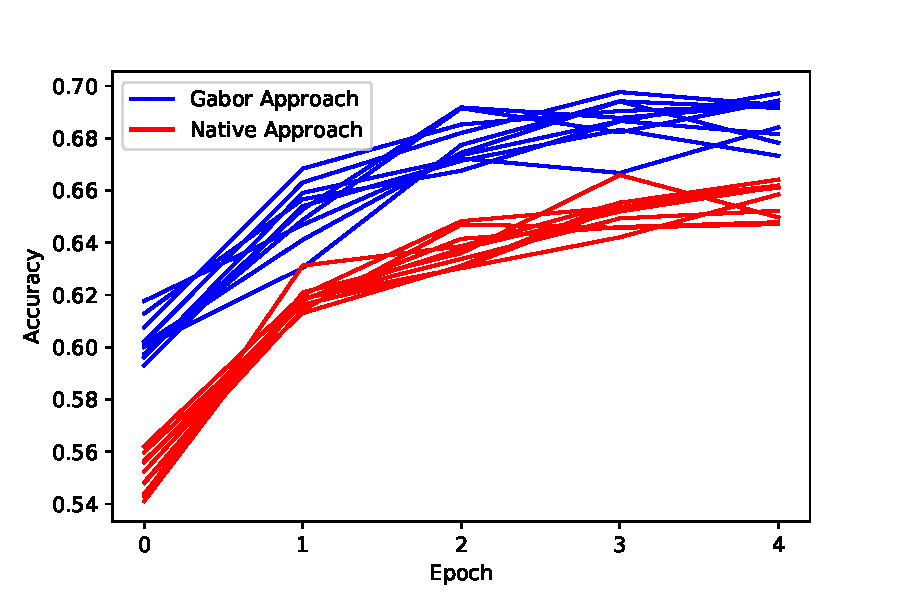
\includegraphics[width=0.7\linewidth]{./papers/visuell/images/accuracy}
	\caption{Test-Genauigkeit (Accuracy) der beiden Varianten im Laufe des Trainings.}
	\label{fig:acc}
\end{figure}

Entscheidend bei neuronalen Netzen sind neben der Genauigkeit die Geschwindigkeiten für das Trainieren und Klassifizieren.
Bei der Variante mit Gabor dauerte das Training etwa 3 Minuten und 10 Sekunden (kann abhängig vom Computer und Grafikkarte stark variieren).
Bei der zweiten Variante, wo erste Layer ebenfalls gelernt wird, dauert das Training ca. 15\% länger (also etwa 3 Minuten und 38 Sekunden).
Das Klassifizieren von neuen Bildern dauert danach bei beiden Varianten gleich lange, da in beiden Fällen die identische Tensorflow-Struktur implementiert wurde.

Lernt das klassische CNN Kernels welche Ähnlichkeiten zu Gabor-Wavelets aufweisen?
In unserem Versuch ist dies nicht der Fall.
Die Kernel welche gelernt wurden sehen zufällig aus, es sind keine Regelmässigkeiten zu erkennen.
Abbildung \ref{fig:cnnkernels} zeigt diese gelernten Kernels, welche mit den Gabor-Kernels in Abbildung \ref{fig:cnngkernels} verglichen werden sollten.
Durch die zufällige Initialisierung ist es aber nicht ausgeschlossen, dass solche Gabor-Ähnlichen Kernels gelernt werden könnten.
Es gibt Beispiele von CNN-Kernels, welche Ähnlichkeiten zu Gabor-Kernels aufweisen (vgl. Kapitel 9.10 im Buch \cite{book:deeplearning}).
Die Vermutung liegt nahe, dass durch die kleine Auflösung der CIFAR-10 Bilder solch komplexe Kernels nicht gelernt wurden.

\begin{figure}
	\centering
	\subfigure{
\includegraphics[width=0.3\linewidth]{./papers/visuell/images/kernel1}}
	\subfigure{
\includegraphics[width=0.3\linewidth]{./papers/visuell/images/kernel2}}
	\subfigure{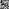
\includegraphics[width=0.3\linewidth]{./papers/visuell/images/kernel3}}
	\caption{Drei verschiedene Kernels des ersten Layers welche vom Netzwerk gelernt wurden. Es sind keine Regelmässigkeiten erkennbar.}
	\label{fig:cnnkernels}
\end{figure}

\begin{figure}
	\centering
	\subfigure{
\includegraphics[width=0.3\linewidth]{./papers/visuell/images/kernelG1}}
	\subfigure{
\includegraphics[width=0.3\linewidth]{./papers/visuell/images/kernelG2}}
	\subfigure{
\includegraphics[width=0.3\linewidth]{./papers/visuell/images/kernelG3}}
	\caption{Drei verschiedene Gabor-Kernels des ersten Layers.}
	\label{fig:cnngkernels}
\end{figure}


